\documentclass[a4paper, 11pt]{article}
\usepackage[T1]{fontenc}
\usepackage[utf8]{inputenc}
\usepackage[norsk]{babel}
\usepackage{graphicx}
\usepackage[dvipsnames]{xcolor}
\usepackage[fleqn]{amsmath}
\usepackage{amsthm}
\usepackage{amssymb}
\usepackage{microtype}
\usepackage{array}
\usepackage{caption}
\usepackage{subcaption}
\usepackage[norsk]{babel}
\usepackage[all]{nowidow}
\usepackage{fancyhdr}
\usepackage{mathtools}
\usepackage{sectsty}

\usepackage{tikz}
\usetikzlibrary{calc,arrows,patterns}
\usepackage{pgfplots}

\usepackage{cancel}
\usepackage{listings}
\usepackage{inconsolata}

% Unicode-inkompatibilitet mactex/texlive?
\DeclareUnicodeCharacter{00A0}{ }

% Få fancyhdr til å holde kjeft
\setlength{\headheight}{14pt} 

\newcommand{\tittel}{Øving 3}
\newcommand{\fag}{Diskret Matematikk}
\newcommand{\fagkode}{TMA4140}
\newcommand{\forfatter}{Steffen Haug}

\renewcommand{\qedsymbol}{$\themecolor{\blacksquare}$}
\newcommand{\ceq}[2]{\stackrel{\text{\tiny{#1}}}{#2}}
\newcommand{\R}{\mathbb{R}}
\newcommand{\deloppg}[1]{\vspace{1mm}\noindent \textbf{\themecolor{#1:}}}
\newcommand{\dint}{\int\displaylimits}

\newcommand{\themeshade}{Mahogany}
\newcommand{\themecolor}[1]{\textcolor{\themeshade}{#1}}
\sectionfont{\color{\themeshade}}

\def\dul#1{\underline{\underline{#1}}}

% Forside
\newcommand*{\titleTH}{\begingroup 
    \raggedleft
    \vspace*{\baselineskip}
    {\Large \forfatter}\\[0.167\textheight]
    {\LARGE\bfseries \tittel}\\[\baselineskip]
    {\themecolor{\Huge \fag}}\\[\baselineskip]
    {\Large \textit{\fagkode}}\par
    \vfill
\endgroup}

\begin{document}

% Front Page
\pagestyle{empty}
\titleTH
\newpage

\lstdefinestyle{themecode}{
    keywordstyle=\themecolor,
}

\lstset{numbers=left, basicstyle=\ttfamily, style=themecode}


\section{Oppgåver til seksjon 3.1}

\subsection*{Oppgåve 53}
Bruker grådig algoritme for myntveksling (Algoritme 6). I staden for å jobbe gjennom
algoritma ``for hand'' brukar eg eit program:

\begin{lstlisting}[language=Python]
def change(C, n):
    D = []
    for c in C:
        t = 0
        while n >= c:
            t += 1
            n -= c
        D.append(t)
    return tuple(D)
\end{lstlisting}

\deloppg{a} 51 cents vekslast til 2 quarters og 1 cent

\deloppg{b} 69 cents vekslast til 2 quarters, 1 dime, 1 nickel og 4 cents

\deloppg{c} 76 cents vekslast til 3 quarters og 1 cent

\deloppg{d} 60 cents vekslast til 2 quarters og 1 dime

\subsection*{Oppgåve 55}
Brukar same algoritme, {\em utan nickels}, med same mangde cents som i \themecolor{53}.
Brukar same programmet som i \themecolor{53}, med forskjellig {\tt C} 
({\tt C = [25,10,1]}).

\deloppg{a} 51 cents vekslast til 2 quarters og 1 cent

\deloppg{b} 69 cents vekslast til 2 quarters, 1 dime, og 9 cents

\deloppg{c} 76 cents vekslast til 3 quarters og 1 cent

\deloppg{d} 60 cents vekslast til 2 quarters og 1 dime

\subsection*{Oppgåve 56}
Viser med eksempel. Ønsker å konstruere eit tal slik at å veksle til ein 12-cent mynt
etterlét oss med eit tal som ikkje kan fordelast ``fint'' på dei gjenverande tala.
Eit eksempel på eit slikt tal er 4 -- det kan ikkje delast på 10 eller 5. 

Vi prøver å rekne gjennom algoritma for {\tt n = 16}, fordi vi veit at dette 
gjev 4 i rest etter å veksle til ein 12-cent.
\begin{alignat*}{3}
    (i)& \quad &&\mathtt{change(}\{25,12,10,5,1\}, 16 \mathtt{)}
        \rightarrow \{0,1,0,0,4\}, \quad &&\Sigma = 5 \\
    (ii)& &&\mathtt{change (}\{25,10,5,1\}, 16 \mathtt{)}
        \rightarrow \{0,1,1,1\}, &&\Sigma = 3
\end{alignat*}

\noindent Sidan algoritma er grådig finn den ikkje den beste løyinga. Same fordeling som i
\((ii)\) er gyldig i \((i)\), men algoritma finn den ikkje.


\newpage
\section{Oppgåver til seksjon 3.2}

\subsection*{Oppgåve 27}

\deloppg{a} 
\begin{align*}
    &\; (n^3 + n^2 \log n)(\log n + 1) + (17 \log n)(n^3 + 2) \\
    \approx &\; (n^3 + n^2 \log n)(\log n) + (\log n)(n^3) \\
    \approx &\; 2n^3 \log n \\
    \approx &\; n^3 \log  n
\end{align*}

\deloppg{b}
\begin{align*}
    &\; (2^n + n^2)(n^3 + 3^n) \\
    \approx &\; (2^n)(3^n) \\
    \approx &\; 3^n
\end{align*}


\subsection*{Oppgåve 30}
Skal vise at funksjonane er av same orden.

\deloppg{c} \(\left\lfloor x + 1/2 \right\rfloor \text{ og } x\)

\noindent Konstantar er irrellevante, \(\left\lfloor x \right\rfloor\) kan maksimalt variere frå
\(x\) med \(\pm 0.5\), som og er irrelevant når \(x\) aukar.

\vspace{2mm}
\deloppg{e} \(\log_{10} x \text{ og } \log_2 x\)

\noindent Brukar L'Hopital til å vise \(\lim_{x \rightarrow \infty} = K\), altso at uttrykka ikkje
er {\em polynomisk forskjellige}.
\begin{align*}
    \lim_{x \rightarrow \infty} \frac{\log_{10}x}{\log_2 x}
        \;\ceq{L'Hop}{=} \lim_{x \rightarrow \infty} \frac{\frac{1}{x\ln 10}}{\frac{1}{x \ln 2}}
        = \frac{\ln 2}{\ln 10}
        = K
\end{align*}

\newpage
\subsection*{Oppgåve 34}

\deloppg{a} Skal vise at \(3x^2 + x + 1\) er \(\Theta(3x^2)\) ved å finne
konstantar \(C_1, C_2\) og \(k\).
Ein kan (relativt) enkelt finne konstantar til polynom ved å gjette.
Til dømes kan ein gjette at \(4x^2 > 3x^2 + x + 1\) fordi \(x^2 > x + 1\), og dermed
\(3x^2 + x^2 > 3x^2 + (x + 1)\), når \(x\) er stor nok.

Når ein løyser oppgåver på denne måten finn ein antageleg ikkje dei minste moglege verdiane for
\(C_1, C_2\) og \(k\), men det er tidsparande.

\vspace{3mm}
\noindent Fann ved ``gjetting'' \( C_1 = \frac{1}{3}, C_2 = \frac{4}{3}\). 
Løyste \(3x^2 + x + 1 = 4x^2\) og fann \(k = \frac{1}{2} + \sqrt{5}\).

\deloppg{b}
\begin{figure}[h]
    \centering
    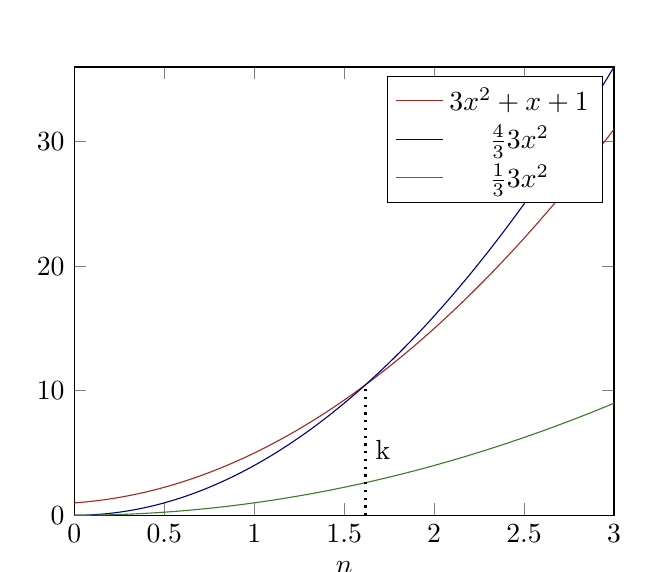
\begin{tikzpicture}
        \begin{axis}[
		xlabel=$n$,
                enlargelimits=false
	]
            \addplot [
                Mahogany,
                domain=0:3,
                samples=200
            ]
                {3*(x^2)+x+1};
            \addplot [
                NavyBlue,
                domain=0:3,
                samples=200
            ]
                {(4/3)*3*x^2};
            \addplot [
                OliveGreen,
                domain=0:3,
                samples=200
            ]
                {(1/3)*(3*x^2)};
            \legend{$3x^2 + x + 1$, $\frac{4}{3}3x^2$, $\frac{1}{3}3x^2$}
            \draw[thick,dotted] (axis cs:1.6180,0) -- (axis cs:1.6180,10.4718) node[midway, right]{k};
	\end{axis}
    \end{tikzpicture}
\end{figure}

\newpage
\subsection*{Oppgåve 42}
Skal undersøkje om \(f(x) \text{ er } O(g(x)) \implies 2^{f(x)} \text{ er } O(2^{g(x)})\).
Prøver med moteksempel.

\begin{align*}
    & \frac{2^{x^2 + x + 1}}{C2^{x^2}} = \frac{2^{x^2}2^x2}{C2^{x^2}}
        = \frac{2^{x+1}}{C} \xrightarrow{x \rightarrow \infty} \infty \\
\end{align*}

\noindent Påstanden held ikkje.



\section{Oppgåver til seksjon 4.1}

\subsection*{Oppgåve 11}
\deloppg{a} 11:00 $+$ 80 timar $=$ 07:00

\deloppg{b} 12:00 $-$ 40 timar $=$ 08:00

\deloppg{c} 06:00 $+$ 100 timar $=$ 10:00

\end{document}
